\documentclass[10pt,a4paper]{article}

\usepackage[a4paper,left=1.35cm,right=1.35cm,top=1.9cm,bottom=1.7cm]{geometry}
\usepackage{amsmath,amssymb,mathtools}
\usepackage[T1]{fontenc}
\usepackage{lmodern}
\usepackage{microtype}
\usepackage{xcolor}
\usepackage{enumitem}
\usepackage{fancyhdr}
\usepackage[most]{tcolorbox}
\usepackage{adjustbox}
\usepackage{tikz}
\usetikzlibrary{arrows.meta,decorations.pathreplacing}
\usepackage{eso-pic}
\usepackage[hidelinks]{hyperref}

\definecolor{boxline}{RGB}{75,75,75}
\definecolor{rulegray}{RGB}{120,120,120}

\newtcolorbox{handbox}{
  enhanced, colback=white, colframe=boxline, boxrule=0.6pt,
  arc=0.8mm, left=3pt, right=3pt, top=2pt, bottom=2pt,
  before skip=3pt, after skip=3pt
}
\newtcolorbox{ideabox}[1][]{
  enhanced, colback=black!3, colframe=black!40, boxrule=0.5pt,
  arc=0.6mm, left=5pt, right=5pt, top=3pt, bottom=3pt,
  fonttitle=\bfseries\small, title={#1}
}

\pagestyle{fancy}
\fancyhf{}
\fancyhead[L]{\small Phy 324 --- Numerical Methods}
\fancyhead[R]{\small Pages 15--29: notes with explanation}
\fancyfoot[C]{\small\thepage}
\renewcommand{\headrulewidth}{0.4pt}

\setlength{\parindent}{0pt}
\setlength{\parskip}{3.2pt}
\setlength{\columnsep}{0.9cm}
\setlength{\abovedisplayskip}{3pt}
\setlength{\belowdisplayskip}{3pt}
\setlength{\abovedisplayshortskip}{1pt}
\setlength{\belowdisplayshortskip}{1pt}
\setlist[itemize]{leftmargin=1.1em,itemsep=0.5pt,topsep=1.5pt,parsep=0pt}
\setlist[enumerate]{leftmargin=1.4em,itemsep=0.5pt,topsep=1.5pt,parsep=0pt}

\newcommand{\fiteq}[1]{\par\noindent\adjustbox{max width=\linewidth}{$\displaystyle #1$}\par}
\newcommand{\fitblock}[1]{\adjustbox{max width=\linewidth}{#1}}

% one original page = two side-by-side columns
\newcommand{\pairpage}[3]{%
  \clearpage
  \section*{\normalsize Page #1}
  \vspace{-0.9em}
  {\color{black!35}\rule{\linewidth}{0.4pt}}\par\vspace{0.2em}
  \noindent
  \begin{minipage}[t]{0.473\textwidth}
    {\scriptsize\textsc{Original notes}}\par\vspace{0.15em}
    {\color{black!25}\rule{\linewidth}{0.3pt}}\par\vspace{0.2em}
    #2
  \end{minipage}%
  \hfill
  \begin{minipage}[t]{0.473\textwidth}
    {\scriptsize\textsc{What is going on}}\par\vspace{0.15em}
    {\color{black!25}\rule{\linewidth}{0.3pt}}\par\vspace{0.2em}
    #3
  \end{minipage}%
}

\begin{document}

\begin{titlepage}
\centering
\vspace*{2.2cm}
{\Huge\bfseries Numerical Methods\par}
\vspace{0.4cm}
{\LARGE Notes, pages 15--29\par}
\vspace{0.5cm}
{\Large with an explanation beside every page\par}
\vspace{1.6cm}

\begin{minipage}{0.78\textwidth}
\begin{ideabox}[How to read this document]
Every page is split into two columns by a vertical line.
\begin{itemize}
\item \textbf{Left:} the contents of the handwritten notes, page by page,
transcribed as faithfully as possible, with the diagrams redrawn.
\item \textbf{Right:} a plain-language explanation of what the notes are
doing, why each step is there, and what the result means.
\end{itemize}
Where the handwriting contains a sign or algebra slip, the right-hand
column points it out and gives the corrected statement; the left-hand
column keeps the original.
\end{ideabox}
\end{minipage}

\vfill
{\small Transcription and commentary of \texttt{01.pdf}, pages 15--29.}
\end{titlepage}

% vertical rule between the two columns, on every page after the title
\AddToShipoutPictureBG{%
  \AtTextCenter{\put(0,-0.5\textheight){\rule{0.4pt}{\textheight}}}%
}

%============================================================
\pairpage{15 --- From an ODE to Euler's method}{%
\begin{itemize}
\item Linear ODE
\item $2$nd order non-linear ODEs
\item PDE's
\item Stochastic systems
\end{itemize}
\[
\frac{dy}{dt}=F(y,t)
\]
Discretize:
\[
\frac{y(t+\Delta t)-y(t)}{\Delta t}=f(y,t)
\]
\[
\lim_{\Delta t\to0}\frac{y(t+\Delta t)-y(t)}{\Delta t}=\frac{dy}{dt}
\]
\begin{handbox}
\[
y(t+\Delta t)=y(t)+\Delta t\,F
\]
\end{handbox}
\begin{center}
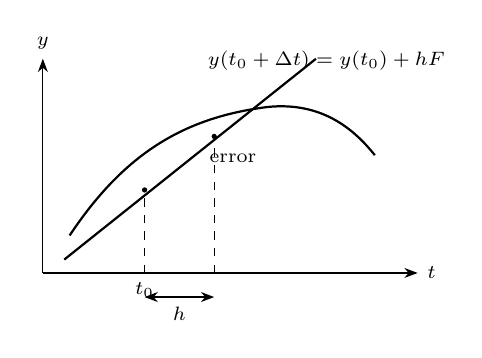
\begin{tikzpicture}[scale=0.68,>=Stealth]
  \draw[->] (0,0)--(7,0) node[right] {\scriptsize $t$};
  \draw[->] (0,0)--(0,4) node[above] {\scriptsize $y$};
  \draw[thick] (0.5,0.7) .. controls (1.5,2.2) and (2.6,2.9) .. (4.2,3.1)
    .. controls (5.2,3.2) and (5.8,2.7) .. (6.2,2.2);
  \draw[thick] (0.4,0.25)--(5.1,4.0);
  \draw[dashed] (1.9,0)--(1.9,1.55);
  \draw[dashed] (3.2,0)--(3.2,2.55);
  \node[below] at (1.9,0) {\scriptsize $t_0$};
  \draw[<->] (1.9,-0.45)--(3.2,-0.45) node[midway,below] {\scriptsize $h$};
  \fill (1.9,1.55) circle (1.4pt);
  \fill (3.2,2.55) circle (1.4pt);
  \node[above right] at (2.9,3.6) {\scriptsize $y(t_0+\Delta t)=y(t_0)+hF$};
  \node at (3.55,2.15) {\scriptsize error};
\end{tikzpicture}
\end{center}
$\to$ Simple Euler method:
\[
y(t_0+h)=y_1=y_0+hf_0
\qquad \left(\text{Error}:O(h^2)\right)
\]
Taylor expansion:
\[
y(t_0+h)=y(t_0)+h\,y'(t_0)+\frac{h^2}{2!}y''(c)
\]
}{%
\textbf{The big idea.} An ODE gives the slope at every point. A computer
cannot take a limit, so it takes a finite step instead:
\[
\frac{y(t+\Delta t)-y(t)}{\Delta t}\approx F(y,t).
\]
Solving for the unknown value gives
$y(t+\Delta t)=y(t)+\Delta t\,F$: follow the tangent line for a time
$\Delta t$. That is \emph{explicit Euler}.

\textbf{The picture.} The straight line is the tangent prediction. The
curved line is the true solution. They start together at $t_0$ and
separate because the true slope changes while Euler keeps using the old
slope. The gap labelled ``error'' is the price of the straight-line
approximation.

\textbf{Where $O(h^2)$ comes from.} Taylor's theorem says
\[
y(t_0+h)=y(t_0)+h y'(t_0)+\frac{h^2}{2}y''(c).
\]
Euler keeps the first two terms and throws away
$\frac{h^2}{2}y''(c)$. So the error made in \emph{one} step is
proportional to $h^2$ (with $h=\Delta t$).

\textbf{Why it is called simple/first-order.} It uses only evaluations
of $F$, never $F'$, so it is easy to program; but its overall accuracy
is only first order, as the next page shows.

\textbf{The list at the top} is just the course map: linear ODEs first,
then nonlinear and second-order ODEs, then PDEs, then stochastic
systems.
}

%============================================================
\pairpage{16 --- Local error, global error, and step size}{%
\[
y_2=y_1+hf_1\qquad\left(\text{Error}\propto O(h^2)\right)
\]
\[
\vdots
\]
\[
y_N=y_{N-1}+hF_{N-1}\qquad\left[\text{Error}:N\,O(h^2)\right]
\]
\[
\text{Local error}: O(h^2)
\]
\[
\text{Global error}: N\,O(h^2)
\]
\[
\begin{cases}
N-\text{No.\ of iterations}\\
T-\text{Total time of solving}\\
\Rightarrow T=Nh
\end{cases}
\]
\[
\text{Global error}:\frac{T}{h}O(h^2)\propto O(h)
\]
\[
\text{Local error}\ll\text{Global error}
\]
\begin{center}
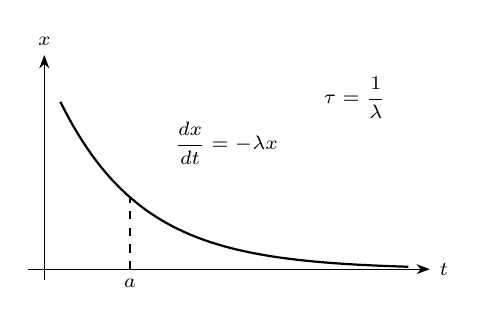
\begin{tikzpicture}[scale=0.68,>=Stealth]
  \draw[->] (-0.3,0)--(7.2,0) node[right] {\scriptsize $t$};
  \draw[->] (0,-0.2)--(0,4.0) node[above] {\scriptsize $x$};
  \draw[thick,domain=0.3:6.8,samples=80] plot (\x,{3.8*exp(-0.65*\x)});
  \draw[dashed] (1.6,0)--(1.6,{3.8*exp(-1.04)});
  \node[below] at (1.6,0) {\scriptsize $a$};
  \node at (3.4,2.35) {\scriptsize $\dfrac{dx}{dt}=-\lambda x$};
  \node at (5.8,3.2) {\scriptsize $\tau=\dfrac{1}{\lambda}$};
\end{tikzpicture}
\end{center}
Choose $\Delta t\ll\tau$ (smaller than the time scale of the problem).

\# How to set $h/\Delta t$?
\begin{enumerate}
\item Convergence
\item Characteristic scales in the system
\end{enumerate}
}{%
\textbf{Two different errors.}
\begin{itemize}
\item \emph{Local error} is the mistake in one step: $O(h^2)$.
\item \emph{Global error} is the mistake at the end after
$N=T/h$ steps. The $N$ small errors add up:
\[
N\cdot O(h^2)=\frac{T}{h}O(h^2)=O(h).
\]
\end{itemize}
So Euler is a \emph{first-order} method globally, even though each step
looks second-order accurate. This is why one should never judge a method
by a single step.

\textbf{Why $N=T/h$.} To integrate from $0$ to $T$ with step $h$ you need
$N=T/h$ steps. The total time is fixed; making $h$ smaller means more
steps, but each step's error falls faster than the number of steps
grows.

\textbf{Choosing the step.} For
$\dot x=-\lambda x$, the solution decays as $e^{-\lambda t}$ and changes
appreciably over the time scale
\[
\tau=\frac{1}{\lambda}.
\]
If $\Delta t$ is comparable to or larger than $\tau$, the tangent step
overshoots the curve, and the numerical solution can oscillate or go
negative. The first rule is therefore $\Delta t\ll\tau$.

\textbf{The second rule.} Always refine: halve the step and check that
the answer stops changing. That is the practical meaning of
``convergence''. The two criteria are (1) the scheme is stable and
convergent, and (2) $\Delta t$ resolves the fastest time scale present.
}

%============================================================
\pairpage{17 --- Nonlinear ODE and fixed points}{%
\textbf{\underline{Non linear ODE:}}
\[
\frac{dx}{dt}=x(1-x^2)
\]
\begin{center}
\begin{tikzpicture}[scale=0.78,>=Stealth]
  \draw[->] (-2.2,0)--(2.4,0) node[right] {\scriptsize $x$};
  \draw[->] (0,-2.2)--(0,2.4) node[above] {\scriptsize $\dot x$};
  \draw[thick,domain=-1.55:1.55,samples=100] plot (\x,{\x*(1-\x*\x)});
  \node[below] at (-1,-0.2) {\scriptsize $-1$};
  \node[below] at (0.05,-0.2) {\scriptsize $0$};
  \node[below] at (1,-0.2) {\scriptsize $+1$};
\end{tikzpicture}
\end{center}
Steady state:
\[
\frac{dx}{dt}=x(1-x^2)=0
\;\Rightarrow\; x=0,\ \pm1
\]
From the graph, given any initial condition $x_0$, we can tell which
steady state the solution will settle to, without knowing the closed
form solution.

If you start close to a steady state and end up diverging away
$\Rightarrow$ unstable steady state; else $\to$ stable steady state.

\textbf{(Double well potential):}
\[
V=\frac12kx^2-\frac14\lambda x^4
\]
\[
m\ddot x=-\gamma\dot x-\frac{\partial V}{\partial x}
\]
For $m/\gamma\ll1$, the second ODE reduces to
$\gamma\dot x=-\partial V/\partial x$. Letting $\gamma=1$:
\[
\dot x=x(1-x^2)
\]
\textbf{2 Dimensional System:}
\[
\frac{dx}{dt}=f(x,y)\ ;\qquad \frac{dy}{dt}=g(x,y)
\]
\[
f(x^*,y^*)=0=g(x^*,y^*)
\]
}{%
\textbf{A flow on a line.} The right-hand side $f(x)=x(1-x^2)$ tells you
the velocity at each $x$. Zeros of $f$ are places where the velocity is
zero: the \emph{fixed points} $x^*=0,\pm1$.

\textbf{Reading stability from the sign.}
\begin{itemize}
\item For $x<-1$: $x<0$ and $1-x^2<0$, so $f>0$; the state moves right,
towards $-1$. For $-1<x<0$: $f<0$; it moves left, also towards $-1$.
Hence $x=-1$ is stable.
\item For $0<x<1$: $f>0$, so it moves right, away from $0$. For
$-1<x<0$: $f<0$, so it moves left, away from $0$. Hence $0$ is unstable.
\item Similarly $x=+1$ is stable: on $(0,1)$ it moves right towards $1$,
and for $x>1$ it moves left towards $1$.
\end{itemize}
The quick test is $f'(x^*)$: negative means stable, positive means
unstable.

\textbf{The potential picture.} A gradient flow
$\gamma\dot x=-V'(x)$ is a particle rolling downhill in $V$. The flow
$x(1-x^2)$ comes from
\[
V(x)=-\frac{x^2}{2}+\frac{x^4}{4},
\]
whose minima are at $x=\pm1$ and whose maximum is at $0$. The notes
write $V=+\frac12kx^2-\frac14\lambda x^4$; with positive $k,\lambda$ that
potential has a well at $0$, not a double well. There is a sign slip:
for the stated flow the quadratic term must be negative.

\textbf{2D systems} are the same idea with two variables: fixed points
solve $f=g=0$, and the sign/eigenvalue analysis decides stability.
}

%============================================================
\pairpage{18 --- Linearising a 2D system}{%
\[
\left.\begin{aligned}
x&=u+x^*\\
y&=v+y^*
\end{aligned}\right\}
\ \to\ \text{perturbations in }x^*\text{ and }y^*
\]
\[
\frac{d}{dt}(u+x^*)=f(u+x^*,v+y^*)
\]
\[
\frac{d}{dt}(v+y^*)=g(u+x^*,v+y^*)
\]
\fiteq{
\frac{\partial u}{\partial t}
=f(x^*,y^*)+\underbrace{u f_x+v f_y}_{0}
}
\fiteq{
\frac{\partial v}{\partial t}
=g(x^*,y^*)+\underbrace{u g_x+v g_y}_{0}
}
\fiteq{
\Rightarrow\quad
\frac{d}{dt}\begin{bmatrix}u\\v\end{bmatrix}
=
\begin{bmatrix}f_x&f_y\\g_x&g_y\end{bmatrix}
\begin{bmatrix}u\\v\end{bmatrix}
}
$\hookrightarrow$ Linearization
\[
J=\begin{bmatrix}a&b\\c&d\end{bmatrix}
=\text{Jacobian}
\]
If $\lambda_1,\lambda_2$ are eigenvalues of $J$:
\[
\begin{bmatrix}u\\v\end{bmatrix}=X
=\alpha v_1e^{\lambda_1t}+\beta v_2e^{\lambda_2t}
\]
\[
\lambda_i\to\text{eigenvalues}\ ;\qquad v_i\to\text{eigenvectors}
\]
}{%
\textbf{Perturb and linearise.} Put the state near a fixed point:
$x=x^*+u$, $y=y^*+v$, with $u,v$ small.

\textbf{Taylor expand.} For example
\fiteq{
f(x^*+u,y^*+v)=f(x^*,y^*)
+u f_x+v f_y+\text{(quadratic terms)}.
}
The constant term vanishes because $(x^*,y^*)$ is a fixed point. For
small perturbations the quadratic terms are negligible, so the
nonlinear system is replaced by the linear system
\[
\dot u=a u+b v,\qquad \dot v=c u+d v.
\]

\textbf{The Jacobian.} The matrix
$J=\begin{bmatrix}f_x&f_y\\g_x&g_y\end{bmatrix}$, evaluated at the fixed
point, is the multivariable analogue of the derivative. Near the point,
the nonlinear flow looks like its linearisation.

\textbf{Eigenvalues tell the story.} The general solution is a
superposition of $e^{\lambda_1t}v_1$ and $e^{\lambda_2t}v_2$.
\begin{itemize}
\item Real $\lambda<0$: that mode decays.
\item Real $\lambda>0$: that mode grows.
\item Complex $\lambda=\alpha\pm i\beta$: oscillation $e^{i\beta t}$
multiplied by growth/decay $e^{\alpha t}$.
\end{itemize}
So the fixed point is stable exactly when both eigenvalues have
negative real parts. The eigenvectors give the directions along which
the motion is purely exponential.
}

%============================================================
\pairpage{19 --- Eigenvalues, trace and determinant}{%
\begin{center}
\begin{tikzpicture}[scale=0.75,>=Stealth]
  \draw[->] (-2.3,0)--(2.3,0) node[right] {\scriptsize $v_1$};
  \draw[->] (0,-2.3)--(0,2.3) node[above] {\scriptsize $v_2$};
  \draw[->] (1.9,0)--(0.6,0); \draw[->] (-1.9,0)--(-0.6,0);
  \draw[->] (0,1.9)--(0,0.6); \draw[->] (0,-1.9)--(0,-0.6);
  \node at (1.75,0.45) {\scriptsize $\lambda_1<0$};
  \node at (0.55,1.95) {\scriptsize $\lambda_2<0$};
\end{tikzpicture}
\end{center}
\[
|J-\lambda I|=
\begin{vmatrix}
a-\lambda&b\\ c&d-\lambda
\end{vmatrix}=0
\]
\[
\Rightarrow\ \lambda^2-(a+d)\lambda+ad-bc=0
\]
\[
\Rightarrow\ \lambda^2-\operatorname{tr}(J)\lambda+\det(J)=0
\]
\[
\Rightarrow\ \lambda=
\frac{\operatorname{tr}(J)\pm
\sqrt{(\operatorname{tr}J)^2-4\det J}}{2}
\]
Let $\operatorname{tr}(J)=\tau$, $\det J=\Delta$:
\[
\lambda_{1,2}=\frac{\tau\pm\sqrt{\tau^2-4\Delta}}{2}
\]
\textbf{CASE I:} $\Delta<0$ ; $\tau>0$
\[
\sqrt{\tau^2-4\Delta}>\tau>0
\]
\[
\hookrightarrow \lambda_1>0\ ;\quad \lambda_2<0
\]
\begin{center}
\begin{tikzpicture}[scale=0.62,>=Stealth]
  \draw[->] (-2.4,0)--(2.4,0) node[right] {\scriptsize $v_1$};
  \draw[->] (0,-2.4)--(0,2.4) node[above] {\scriptsize $v_2$};
  \draw[->] (0.3,0)--(1.9,0); \draw[->] (-0.3,0)--(-1.9,0);
  \draw[->] (0,1.7)--(0,0.4); \draw[->] (0,-1.7)--(0,-0.4);
\end{tikzpicture}
\end{center}
}{%
\textbf{From the matrix to a quadratic.}
\[
\det(J-\lambda I)=0
\]
gives
\[
\lambda^2-(a+d)\lambda+(ad-bc)=0.
\]
Two combinations appear:
\[
\tau=a+d=\lambda_1+\lambda_2
\quad\text{(trace)},
\]
\[
\Delta=ad-bc=\lambda_1\lambda_2
\quad\text{(determinant)}.
\]
So the eigenvalues are
\[
\lambda_{1,2}=\frac{\tau\pm\sqrt{\tau^2-4\Delta}}{2}.
\]
This is just the quadratic formula; it lets you classify a fixed point
from two numbers without computing eigenvectors.

\textbf{The discriminant decides the type.}
\[
\tau^2-4\Delta
\]
is the square of the difference of the eigenvalues.
\begin{itemize}
\item Positive: two distinct real eigenvalues (node or saddle).
\item Zero: repeated real eigenvalue (degenerate node).
\item Negative: complex conjugate pair (spiral or centre).
\end{itemize}

\textbf{Case I: $\Delta<0$.} The product $\lambda_1\lambda_2$ is
negative, so the eigenvalues have opposite signs: one direction grows,
the other decays. That is a \emph{saddle}. The sketch shows flow out
along $v_1$ and in along $v_2$.

\textbf{The top sketch} is the stable node: both eigenvalues negative,
so all arrows point towards the origin.
}

%============================================================
\pairpage{20 --- Classifying fixed points}{%
\textbf{CASE II:} $\Delta>0$

\textbf{(i)} $\tau^2-4\Delta>0$ ; $\tau>0$
\[
\hookrightarrow \lambda_1,\lambda_2>0
\]
\begin{center}
\begin{tikzpicture}[scale=0.55,>=Stealth]
  \draw[->] (-2.1,0)--(2.1,0) node[right] {\scriptsize $v_1$};
  \draw[->] (0,-2.1)--(0,2.1) node[above] {\scriptsize $v_2$};
  \draw[->] (0.3,0)--(1.7,0); \draw[->] (-0.3,0)--(-1.7,0);
  \draw[->] (0,0.3)--(0,1.7); \draw[->] (0,-0.3)--(0,-1.7);
\end{tikzpicture}
\end{center}
\textbf{(ii)} $\tau^2-4\Delta>0$ ; $\tau<0$
\[
\hookrightarrow \lambda_1,\lambda_2<0
\]
\begin{center}
\begin{tikzpicture}[scale=0.55,>=Stealth]
  \draw[->] (-2.1,0)--(2.1,0) node[right] {\scriptsize $v_1$};
  \draw[->] (0,-2.1)--(0,2.1) node[above] {\scriptsize $v_2$};
  \draw[->] (1.7,0)--(0.3,0); \draw[->] (-1.7,0)--(-0.3,0);
  \draw[->] (0,1.7)--(0,0.3); \draw[->] (0,-1.7)--(0,-0.3);
\end{tikzpicture}
\end{center}
\textbf{(iii)} $\tau^2-4\Delta<0$ ; $\tau>0$
\[
\hookrightarrow \lambda_1,\lambda_2\in\mathbb{C}
\]
\[
\hookrightarrow e^{\tau}e^{i\Box}=\lambda_{\Box}
\]
$\tau>0\Rightarrow$ Anti-damped
\begin{center}
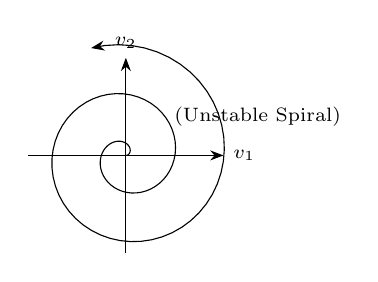
\begin{tikzpicture}[scale=0.62,>=Stealth]
  \draw[->] (-2.0,0)--(2.0,0) node[right] {\scriptsize $v_1$};
  \draw[->] (0,-2.0)--(0,2.0) node[above] {\scriptsize $v_2$};
  \draw[->,domain=0:4.6*pi,samples=120] plot
    ({0.16*\x*cos(\x r)},{0.16*\x*sin(\x r)});
  \node at (2.7,0.8) {\scriptsize (Unstable Spiral)};
\end{tikzpicture}
\end{center}
\textbf{(iv)} $\tau^2-4\Delta<0$ ; $\tau<0$ \quad (Damped Spiral)
\begin{center}
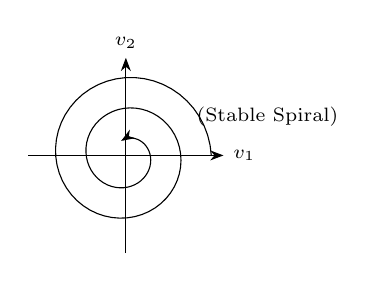
\begin{tikzpicture}[scale=0.62,>=Stealth]
  \draw[->] (-2.0,0)--(2.0,0) node[right] {\scriptsize $v_1$};
  \draw[->] (0,-2.0)--(0,2.0) node[above] {\scriptsize $v_2$};
  \draw[->,domain=0:4.6*pi,samples=120] plot
    ({1.75*(1-\x/(5.6*pi))*cos(\x r)},
     {1.75*(1-\x/(5.6*pi))*sin(\x r)});
  \node at (2.9,0.8) {\scriptsize (Stable Spiral)};
\end{tikzpicture}
\end{center}
}{%
\textbf{$\Delta>0$: both eigenvalues have the same sign.} The sign of
$\tau=\lambda_1+\lambda_2$ then decides whether both are positive or both
negative. The discriminant decides whether they are real or complex.

\textbf{Real eigenvalues.}
\begin{itemize}
\item[(i)] $\tau>0$: both positive. Every direction grows.
An \emph{unstable node}. Arrows point away.
\item[(ii)] $\tau<0$: both negative. Every direction decays.
A \emph{stable node}. Arrows point in.
\end{itemize}

\textbf{Complex eigenvalues.} Write
$\lambda=\alpha\pm i\beta$ with
$\alpha=\tau/2$, $\beta=\sqrt{4\Delta-\tau^2}/2$. The solution is
$e^{\alpha t}(\cos\beta t,\sin\beta t)$: rotation at rate $\beta$ with
amplitude changing as $e^{\alpha t}$.
\begin{itemize}
\item[(iii)] $\tau>0$: $\alpha>0$, amplitude grows. An
\emph{unstable spiral} (the notes call it ``anti-damped'').
\item[(iv)] $\tau<0$: $\alpha<0$, amplitude decays. A
\emph{stable spiral} (``damped'').
\item[(v)] (next page) $\tau=0$: $\alpha=0$, constant amplitude. A
\emph{centre}; the orbits are closed.
\end{itemize}

\textbf{The one-line summary.}
\[
\begin{aligned}
\Delta<0 &: \text{saddle},\\
\Delta>0,\ \tau<0 &: \text{stable},\\
\Delta>0,\ \tau>0 &: \text{unstable}.
\end{aligned}
\]
The discriminant then refines ``node'' versus ``spiral''. In tabular
form:
\[
\begin{array}{c|c|c}
\Delta & \tau & \text{type}\\ \hline
<0 & \text{any} & \text{saddle}\\
>0 & <0 & \text{stable}\\
>0 & >0 & \text{unstable}\\
>0 & =0 & \text{centre}
\end{array}
\]
and, when $\Delta>0$,
\[
\tau^2-4\Delta
\begin{cases}
>0: & \text{node},\\
<0: & \text{spiral}.
\end{cases}
\]
}

%============================================================
\pairpage{21 --- A worked example, then PDEs}{%
{\footnotesize
\textbf{(v)} $\tau^2-4\Delta<0$ ; $\tau=0$
\begin{center}
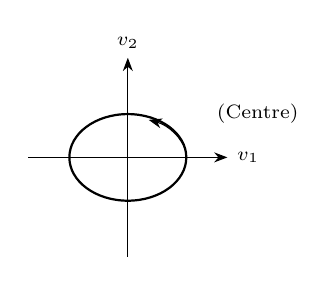
\begin{tikzpicture}[scale=0.55,>=Stealth]
  \draw[->] (-2.3,0)--(2.3,0) node[right] {\scriptsize $v_1$};
  \draw[->] (0,-2.3)--(0,2.3) node[above] {\scriptsize $v_2$};
  \draw[thick] (0,0) ellipse (1.35 and 1.0);
  \draw[->] (1.35,0.1) arc (10:70:1.35 and 1.0);
  \node at (3.0,1.0) {\scriptsize (Centre)};
\end{tikzpicture}
\end{center}
\textbf{(vi)}
\[
\dot x=x(3-x-2y),\qquad \dot y=y(2-x-y)
\]
\[
0=x(3-x-2y),\qquad 0=y(2-x-y)
\]
\[
3-x-2y=0
\]
\begin{handbox}
\[
\begin{array}{cc}
\boxed{x=y=0} & \boxed{y=0,\ x=3}\\[3pt]
\boxed{x=0,\ y=2} &\\[2pt]
\boxed{x=y=1} &
\end{array}
\]
\end{handbox}
\textbf{Partial differential eqn}
\[
\frac{\partial P}{\partial t}=F(P,t),\qquad
\frac{\partial P}{\partial t}=D\frac{\partial^2P}{\partial x^2}
\]
\begin{center}
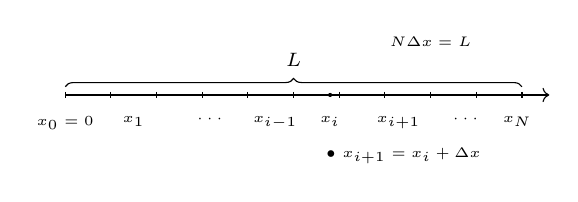
\begin{tikzpicture}[scale=0.58]
  \draw[->] (0,0)--(10.6,0);
  \foreach \x in {0,1,...,10} \draw (\x,0.07)--(\x,-0.07);
  \node[below] at (0,-0.25) {\tiny $x_0=0$};
  \node[below] at (1.5,-0.25) {\tiny $x_1$};
  \node[below] at (3.2,-0.25) {\tiny $\cdots$};
  \node[below] at (4.6,-0.25) {\tiny $x_{i-1}$};
  \node[below] at (5.8,-0.25) {\tiny $x_i$};
  \node[below] at (7.3,-0.25) {\tiny $x_{i+1}$};
  \node[below] at (8.8,-0.25) {\tiny $\cdots$};
  \node[below] at (9.9,-0.25) {\tiny $x_N$};
  \draw[decorate,decoration={brace,amplitude=3pt}] (0,0.18)--(10,0.18);
  \node[above] at (5,0.40) {\scriptsize $L$};
  \node[above] at (8.0,0.85) {\tiny $N\Delta x=L$};
  \fill (5.8,0) circle (1.3pt);
  \node[below] at (7.4,-0.95) {\tiny $\bullet\ x_{i+1}=x_i+\Delta x$};
\end{tikzpicture}
\end{center}
\[
\frac{\partial F}{\partial x}
=\frac{F(x_{i+1})-F(x_i)}{\Delta x}
=\frac{F(x+\Delta x)-F(x)}{\Delta x}
\]
Also:
\[
\frac{\partial F}{\partial x}
=\frac{F(x_i)-F(x_{i-1})}{\Delta x}
=\frac{F(x_{i+1})-F(x_{i-1})}{2\Delta x}
\]
}
}{%
\textbf{The example.} Set both rates to zero:
\[
\dot x=0\ \Rightarrow\ x=0\ \text{or}\ 3-x-2y=0,
\]
\[
\dot y=0\ \Rightarrow\ y=0\ \text{or}\ 2-x-y=0.
\]
Intersections of these \emph{nullclines} give the fixed points:
$(0,0)$, $(0,2)$, $(3,0)$, and $(1,1)$. The last one solves
$3-x-2y=0$, $2-x-y=0$.

\textbf{Then the notes switch to PDEs.} Now $P=P(x,t)$: the unknown
depends on space as well as time. The same finite-difference idea is
applied to the space derivative.

\textbf{The grid.} Choose points
\[
x_i=i\Delta x,\qquad i=0,1,\dots,N,
\]
so that $N\Delta x=L$ covers the interval. $x_{i+1}=x_i+\Delta x$.

\textbf{Three ways to approximate a slope.}
\begin{itemize}
\item Forward: $[F(x_{i+1})-F(x_i)]/\Delta x$.
\item Backward: $[F(x_i)-F(x_{i-1})]/\Delta x$.
\item Central: $[F(x_{i+1})-F(x_{i-1})]/(2\Delta x)$.
\end{itemize}
The central one averages the two one-sided slopes and is more accurate
(second order instead of first order).

\textbf{Why this matters.} Once derivatives are replaced by differences,
a differential equation becomes a set of algebraic equations for the
grid values --- something a computer can solve.
}

%============================================================
\pairpage{22 --- Diffusion: from PDE to update}{%
Coming back to the diffusion equation. Discretize the second
derivative:
\[
\frac{\partial^2F}{\partial x^2}
=\frac{\partial}{\partial x}
\left(\frac{F(x+\Delta x)-F(x)}{\Delta x}\right)
\]
\[
=\frac{F(x+\Delta x)-F(x)-(F(x)-F(x-\Delta x))}{(\Delta x)^2}
\]
\[
=\frac{F(x+\Delta x)-2F(x)+F(x-\Delta x)}{(\Delta x)^2}
\]
\[
\Rightarrow\ 
\frac{P(x,t_n+\Delta t)-P(x,t_n)}{\Delta t}
=D\frac{\partial^2P}{\partial x^2}
\]
\[
P(x,t_n+\Delta t)=P(x,t_n)+D\Delta t\frac{\partial^2P}{\partial x^2}
\]
\fiteq{
=P(x_i,t_n)+\frac{D\Delta t}{\Delta x^2}
\left[P(x_{i+1},t_n)+P(x_{i-1},t_n)-2P(x_i,t_n)\right]
}
\begin{handbox}
\[
P_i^{\,n+1}=P_i^{\,n}
+\frac{D\Delta t}{\Delta x^2}
\left(P_{i+1}^{\,n}+P_{i-1}^{\,n}-2P_i^{\,n}\right)
\]
\end{handbox}
$\hookrightarrow$ Discretization of diffusion.
\[
P_i^{\,n}=T^nX_i
=T^n\sum_{j=1}^{N}e^{ik_jx_i}\hat X_j
\]
\[
f(x)=\int e^{ikx}\hat f(k)\,dk
\]
\begin{handbox}
\centering
$\text{Sol}^n=\text{Temporal}\times\text{Spatial part}$
\end{handbox}
}{%
\textbf{Why the second difference looks like that.} The second
derivative is the derivative of the first derivative. Approximate the
outer derivative by a forward difference and the two inner derivatives
by backward differences:
\[
\partial_x^2F\approx
\frac{F_{i+1}-F_i}{\Delta x}
-\frac{F_i-F_{i-1}}{\Delta x}
\quad\text{all over }\Delta x.
\]
That gives
\[
\frac{F_{i+1}-2F_i+F_{i-1}}{\Delta x^2}.
\]

\textbf{The explicit FTCS scheme.} Use a forward difference in time and
a central difference in space:
\[
P_i^{n+1}=P_i^n+\frac{D\Delta t}{\Delta x^2}
(P_{i+1}^n-2P_i^n+P_{i-1}^n).
\]
``Explicit'' means the new value is written directly in terms of old
values; no linear system has to be solved. If a cell is a peak, the
bracket is negative and the peak decreases; if it is a dip, the bracket
is positive and it fills in. That is diffusion.

\textbf{The Fourier idea.} Any spatial profile can be written as a sum
of waves $e^{ikx}$. The scheme does not mix different $k$'s, so we can
follow one mode at a time. Write
$P_i^n=T^n e^{ikx_i}$: $T^n$ is the amplitude after $n$ steps. If
$|T^{n+1}/T^n|\le1$ for every $k$, no mode grows and the scheme is
stable. The next page computes this ratio and turns it into a condition
on $\Delta t$.
}

%============================================================
\pairpage{23 --- Von Neumann stability}{%
\[
\downarrow\quad\text{In Fourier transform}
\]
Substitute this in the discretization:
\begin{multline*}
T^{n+1}\sum_j e^{ik_jx_i}\hat X_j
=T^n\sum_j e^{ik_jx_i}\hat X_j\\
+\frac{D\Delta t}{\Delta x^2}
\Bigl[T^n\sum_j e^{ik_j(x_i+\Delta x)}\hat X_j
+T^n\sum_j e^{ik_j(x_i-\Delta x)}\hat X_j\\
-2T^n\sum_j e^{ik_jx_i}\hat X_j\Bigr]
\end{multline*}
For the $j$th component:
\begin{multline*}
T^{n+1}e^{ik_jx_i}\hat X_j
=T^ne^{ik_jx_i}\hat X_j\\
+C\hat X_jT^n
\left[e^{ik_j(x_i+\Delta x)}+e^{ik_j(x_i-\Delta x)}
-2e^{ik_jx_i}\right]
\end{multline*}
\begin{handbox}
\[
C=-\frac{D\Delta t}{\Delta x^2}
\]
\end{handbox}
\[
\Rightarrow\ T^{n+1}\hat X_j
=T^n\hat X_j+C\hat X_jT^n
\left[e^{ik_j\Delta x}+e^{-ik_j\Delta x}-2\right]
\]
\begin{handbox}
\[
T^{n+1}=T^n\left[1+C(2\cos(k_j\Delta x)-2)\right]
\]
\end{handbox}
\[
\hookrightarrow\ T^{n+1}
=T^n\left[1-4C\sin^2\left(\frac{k_j\Delta x}{2}\right)\right]
\]
We need $T^{n+1}\le T^n$:
\[
\left|1-4C\sin^2\left(\frac{k_j\Delta x}{2}\right)\right|\le1
\]
\[
\hookrightarrow\ -(1-4C)\le1
\quad\Longrightarrow\quad
\boxed{C\le\frac12}
\]
\begin{handbox}
\[
\frac{D\Delta t}{\Delta x^2}\le\frac12
\]
\end{handbox}
\[
\longrightarrow\quad\text{Neumann stability condition}
\]
}{%
\textbf{The calculation.} Insert
$P_i^n=T^n e^{ikx_i}$ into the update. Every term carries the common
factor $e^{ikx_i}$, so it cancels. What remains is an equation for the
amplitude:
\[
T^{n+1}=T^n\left[1+C(2\cos(k\Delta x)-2)\right].
\]
Using $2\cos\theta-2=-4\sin^2(\theta/2)$,
\[
\frac{T^{n+1}}{T^n}
=1-4C\sin^2\left(\frac{k\Delta x}{2}\right),
\qquad C=\frac{D\Delta t}{\Delta x^2}.
\]

\textbf{Stability.} A mode is stable if its amplitude does not grow:
\[
\left|1-4C\sin^2\frac{k\Delta x}{2}\right|\le1
\quad\text{for all }k.
\]
The worst case is $\sin^2=1$, which gives
\[
-1\le1-4C\le1
\quad\Longrightarrow\quad
0\le C\le\frac12.
\]
So
\[
\boxed{\Delta t\le\frac{\Delta x^2}{2D}}.
\]

\textbf{What it means.} In one time step, diffusion must not move
information further than about one grid spacing. If $\Delta t$ is too
large, neighbouring cells over-correct each other and a sawtooth
(alternating $+,-,+,-$) pattern grows without bound.

\textbf{A note on the notes.} The handwritten box says
$C=-D\Delta t/\Delta x^2$, and the inequality line is also written
inconsistently. With the plus sign used in the update, $C$ must be
positive; the correct final condition is the boxed
$D\Delta t/\Delta x^2\le1/2$.
}

%============================================================
\pairpage{24 --- Wave equation and advection}{%
\textbf{\underline{Wave Eqn:}}
\[
\frac{\partial^2\psi}{\partial t^2}
=c^2\frac{\partial^2\psi}{\partial x^2}
\]
\[
\downarrow
\]
\[
\frac{\partial\psi}{\partial t}
=c\frac{\partial\psi}{\partial x}
\]
\fiteq{
\psi=F(x-ct)=e^{-(x-ct)^2}
\qquad\text{(rightward travelling wave)}
}
\[
\frac{\partial\psi}{\partial t}
=e^{-(x-ct)^2}(+2)(x-ct)c
\]
\[
\frac{\partial\psi}{\partial x}
=e^{-(x-ct)^2}(-2)(x-ct)
\]
\[
\hookrightarrow\ 
\frac{\partial\psi}{\partial t}
=-c\frac{\partial\psi}{\partial x}
\qquad\checkmark\quad\text{(works for Gaussian!)}
\]
The second-order equation is not first order with $x-ct$: thus the
backward wave is not a solution to the second-order equation.

Mechanism of wave propagation in second order $\to$ advection.

To describe advection + diffusion:
\begin{handbox}
\[
\frac{\partial P}{\partial t}
=D\frac{\partial^2P}{\partial x^2}
-c\frac{\partial P}{\partial x}
\]
\end{handbox}
}{%
\textbf{Factoring the wave operator.}
\[
\partial_t^2-c^2\partial_x^2
=(\partial_t-c\partial_x)(\partial_t+c\partial_x).
\]
Each factor is a one-way wave equation. The first-order equation
\[
\partial_t\psi=-c\partial_x\psi
\]
describes a shape moving to the right without changing form:
$\psi=f(x-ct)$.

\textbf{Check with a Gaussian.} For
$\psi=e^{-(x-ct)^2}$,
\[
\partial_t\psi=2c(x-ct)e^{-(x-ct)^2},
\]
\[
\partial_x\psi=-2(x-ct)e^{-(x-ct)^2}.
\]
Therefore $\partial_t\psi=-c\partial_x\psi$, as claimed. (The notes
first write $+c$; the correct sign for a right-moving pulse is minus.
The Gaussian check catches it.)

\textbf{Why the second-order equation is different.} It contains both
factors, so it allows right-moving and left-moving waves. The
first-order advection equation keeps only one direction; a left-moving
pulse is not a solution of it.

\textbf{Adding diffusion.} Real transport often has both drift and
spreading:
\[
\partial_tP=D\partial_x^2P-c\partial_xP.
\]
The first term spreads the profile; the second carries it along at
speed $c$.
}

%============================================================
\pairpage{25 --- Upwind advection and stability}{%
\textbf{\underline{Coming back to advection:}}
\[
\frac{\psi_i^{\,n+1}-\psi_i^{\,n}}{\Delta t}
=-c\left(\frac{\psi_i^{\,n}-\psi_{i-1}^{\,n}}{\Delta x}\right)
\]
\[
\Rightarrow\ \psi_i^{\,n+1}
=\psi_i^{\,n}-\frac{c\Delta t}{\Delta x}
\left(\psi_i^{\,n}-\psi_{i-1}^{\,n}\right)
\]
\textbf{Stability condition.}
\[
\psi_i^{\,n}=T^nX_i\ ;\qquad
X_i=\sum_j e^{ik_jx_i}\hat X_j
\]
Substituting:
\begin{multline*}
T^{n+1}\sum_i e^{ik_jx_i}\hat X_j
=T^n\sum_j e^{ik_jx_i}\hat X_j\\
-\frac{c\Delta t}{\Delta x}
\left[T^n\sum_j e^{ik_jx_i}\hat X_j
-T^n\sum_j e^{ik_j(x_i-\Delta x)}\hat X_j\right]
\end{multline*}
For the $j$th mode:
\begin{multline*}
T^{n+1}e^{ik_jx_i}\hat X_j
=T^ne^{ik_jx_i}\hat X_j\\
-\frac{c\Delta t}{\Delta x}
\left[T^ne^{ik_jx_i}\hat X_j
-T^ne^{ik_j(x_i-\Delta x)}\hat X_j\right]
\end{multline*}
\[
T^{n+1}=T^n-\frac{c\Delta t}{\Delta x}
\left[T^n-e^{-ik_j\Delta x}T^n\right]
\]
\begin{handbox}
\[
T^{n+1}=T^n\left[1+e^{-ik_j\Delta x}
\frac{c\Delta t}{\Delta x}-\frac{c\Delta t}{\Delta x}\!\right]
\]
\end{handbox}
Let
\[
K=\frac{c\Delta t}{\Delta x}
\]
}{%
\textbf{Upwind differencing.} For $c>0$ the disturbance comes from the
left. It is therefore natural to approximate the space slope by the
backward difference:
\[
\partial_x\psi\approx\frac{\psi_i-\psi_{i-1}}{\Delta x}.
\]
This is the \emph{upwind} (or donor-cell) scheme:
\[
\psi_i^{n+1}=\psi_i^n-K(\psi_i^n-\psi_{i-1}^n),
\qquad K=\frac{c\Delta t}{\Delta x}.
\]
It is explicit and only first-order accurate; it tends to smear sharp
fronts (numerical diffusion), but it is robust.

\textbf{Fourier analysis.} Put
$\psi_i^n=T^n e^{ikx_i}$. The common exponential cancels, leaving
\[
T^{n+1}=T^n\left[1-K(1-e^{-ik\Delta x})\right].
\]
The quantity in brackets is the amplification factor for the mode $k$.
The next page requires its modulus to be at most $1$ for every $k$.

\textbf{Reading the factor.} For $k\Delta x\ll1$, expand
$e^{-ik\Delta x}\approx1-ik\Delta x$:
\[
1-K(1-e^{-ik\Delta x})\approx1-ikc\Delta t.
\]
That is the first two terms of $e^{-ikc\Delta t}$, i.e.\ the exact
translation by $c\Delta t$. The scheme is trying to move the wave one
cell-velocity step per time step.
}

%============================================================
\pairpage{26 --- CFL condition and wave scheme}{%
\[
T^{n+1}=T^n\left[1-K\left(1-e^{-ik_j\Delta x}\right)\right]
\]
We impose the condition that
\[
\left|1-K\underbrace{\left(1-e^{-ik_j\Delta x}\right)}
_{\text{max val }=2}\right|\le1
\]
\[
\longrightarrow\quad -(2K+1)\le1
\]
\[
\Rightarrow\quad 2K-1\ge1
\]
\[
\Rightarrow\quad \boxed{K\le1}
\]
\begin{handbox}
\[
\frac{C\Delta t}{\Delta x}\le1
\]
{\small $\to$ stability condition for 1st order wave eqn}
\end{handbox}
\begin{handbox}
\[
c\le\frac{\Delta x}{\Delta t}
\]
\end{handbox}
\[
\longrightarrow\quad\text{rate of updating}>\text{velocity}
\]
\textbf{2nd order wave eqn:}
\[
\frac{\psi_i^{\,n+1}+\psi_i^{\,n-1}-2\psi_i^{\,n}}{(\Delta t)^2}
=c^2\left(
\frac{\psi_{i+1}^{\,n}+\psi_{i-1}^{\,n}-2\psi_i^{\,n}}{(\Delta x)^2}
\right)
\]
\[
\begin{aligned}
\psi_i^{\,n+1}={}&\frac{c^2\Delta t^2}{\Delta x^2}
\left(\psi_{i+1}^{\,n}+\psi_{i-1}^{\,n}\right)\\
&+2\left(1-\frac{c^2\Delta t^2}{\Delta x^2}\right)\psi_i^{\,n}
-\psi_i^{\,n-1}
\end{aligned}
\]
}{%
\textbf{The CFL condition.} The amplification factor is
\[
A(k)=1-K(1-e^{-ik\Delta x}).
\]
Its modulus is at most $1$ for every $k$ exactly when
\[
0\le K\le1,
\qquad K=\frac{c\Delta t}{\Delta x}.
\]
Equivalently,
\[
c\Delta t\le\Delta x.
\]
(In the boxed line the notes write $C\Delta t/\Delta x\le1$; there $C$
denotes the wave speed, written $c$ everywhere else.)
This is the Courant--Friedrichs--Lewy (CFL) condition.

\textbf{Physical meaning.} In one time step, the true signal travels a
distance $c\Delta t$. The numerical scheme can only use information
from neighbouring grid points, a distance $\Delta x$. If
$c\Delta t>\Delta x$, the scheme cannot see the data that should
influence the answer, and it becomes unstable. Hence
``rate of updating $>$ velocity''.

\textbf{A note on the handwritten algebra.} The lines
$-(2K+1)\le1$ and $2K-1\ge1$ have sign/index slips; the conclusion
$K\le1$ is correct. The clean derivation is
$|1-K(1-e^{-i\theta})|^2=1-4K(1-K)\sin^2(\theta/2)\le1$ for all
$\theta$, which requires $0\le K\le1$.

\textbf{Second-order wave scheme.} Use central differences in both time
and space:
\fiteq{
\frac{\psi_i^{n+1}-2\psi_i^n+\psi_i^{n-1}}{\Delta t^2}
=c^2\frac{\psi_{i+1}^n-2\psi_i^n+\psi_{i-1}^n}{\Delta x^2}.
}
Solving for the newest level gives the displayed three-level update.
It needs $\psi^0$ and $\psi^1$ to start (next page). It is stable for
the same Courant condition $c\Delta t/\Delta x\le1$; the special value
$K=1$ reproduces the exact solution on a uniform grid.
}

%============================================================
\pairpage{27 --- Starting the wave scheme}{%
\fiteq{
\psi_i^{\,1}
=K^2\left(\psi_{i+1}^{\,0}+\psi_{i-1}^{\,0}\right)
+2(1-K^2)\psi_i^{\,0}-\psi_i^{-1}
}
Initial condition (known):
\[
\left.\frac{\partial\psi}{\partial t}\right|_{t=0}
=\frac{\psi_i^{\,1}-\psi_i^{-1}}{2\Delta t}
\]
\[
\Rightarrow\ -2\Delta t
\left(\left.\frac{\partial\psi}{\partial t}\right|_{t=0}\right)
+\psi_i^{\,1}=\psi_i^{-1}
\]
\begin{handbox}
\[
\therefore\quad \psi_i^{-1}
=\psi_i^{\,1}-2\Delta t
\left(\left.\frac{\partial\psi}{\partial t}\right|_{t=0}\right)
\]
\end{handbox}
\begin{handbox}
\[
\psi_i^{\,1}
=\frac{K^2}{2}\left(\psi_{i+1}^{\,0}+\psi_{i-1}^{\,0}\right)
+(1-K^2)\psi_i^{\,0}
+\Delta t\!\left.\frac{\partial\psi}{\partial t}\right|_{t=0}
\]
\end{handbox}
\[
K=\frac{\Delta x}{\Delta t}
\quad\longrightarrow\quad
\text{exact solution (for 2nd order)}
\]
\begin{ideabox}[Inserted photograph]
Taylor expansions:
\[
\psi(x+\Delta x)=\psi+\Delta x\psi_x
+\frac{\Delta x^2}{2!}\psi_{xx}+\cdots
\]
\[
\psi(x-\Delta x)=\psi-\Delta x\psi_x
+\frac{\Delta x^2}{2!}\psi_{xx}+\cdots
\]
\[
\begin{aligned}
\psi_{xx}={}&\frac{\psi(x+\Delta x)+\psi(x-\Delta x)-2\psi}{\Delta x^2}\\
&-\frac{2\Delta x^2}{4!}\psi_{xxxx}-\cdots
\end{aligned}
\]
Similarly for $\psi_{tt}$ with $\Delta t$.
\end{ideabox}
}{%
\textbf{Why a starter is needed.} The three-level wave scheme computes
level $n+1$ from levels $n$ and $n-1$. At the start we know $\psi^0$
(the initial shape) but not $\psi^1$. The initial \emph{velocity}
supplies the missing information.

\textbf{Using the velocity.} Approximate the initial velocity by a
centred time difference:
\[
\left.\partial_t\psi\right|_{0}
\approx\frac{\psi_i^1-\psi_i^{-1}}{2\Delta t}.
\]
Here $\psi_i^{-1}$ is a fictitious level before $t=0$. Solve for it:
\[
\psi_i^{-1}=\psi_i^1-2\Delta t\,(\partial_t\psi)_0.
\]
Substitute this into the wave update at $n=0$ and solve for $\psi_i^1$.
The result is the boxed first-step formula. It uses $\psi^0$, the
initial velocity, and the same Courant number.

\textbf{The photograph.} It is the Taylor justification for the central
differences. Adding the expansions of $\psi(x+\Delta x)$ and
$\psi(x-\Delta x)$ cancels the first-derivative terms and leaves
\[
\psi_{xx}=\frac{\psi_{i+1}-2\psi_i+\psi_{i-1}}{\Delta x^2}
+O(\Delta x^2).
\]
The same holds in time. That is why the scheme is second-order accurate.

\textbf{The last line.} The notes write $K=\Delta x/\Delta t$. The
dimensionless Courant number for the wave equation is
$K=c\Delta t/\Delta x$; the statement ``exact solution'' refers to the
special case $K=1$, where the numerical grid moves exactly with the
wave.
}

%============================================================
\pairpage{28 --- Fokker--Planck equation}{%
\textbf{\underline{Derivation of Fokker--Planck eqn}}
\[
\frac{\partial P}{\partial t}=-\nabla\cdot\vec J
\qquad\text{(continuity eqn)}
\]
\[
\vec J_{\text{diffusion}}+\vec J_{\text{drift}}=\vec J
\]
\[
\vec J_{\text{diffusion}}
=-D\frac{\partial P}{\partial x}
\]
\[
\vec J_{\text{drift}}
=-P\frac{\partial\Phi}{\partial x}
\]
\begin{handbox}
\[
\frac{\partial P}{\partial t}
=\frac{\partial}{\partial x}
\left[D\frac{\partial P}{\partial x}
+P\frac{\partial\Phi}{\partial x}\right]
\]
\end{handbox}
}{%
\textbf{Conservation of probability.} $P(x,t)$ is a probability density.
The continuity equation
\[
\partial_tP=-\nabla\cdot J
\]
says: the amount of probability in a small region changes only because
probability flows across its boundaries. $J$ is the probability current.

\textbf{Two contributions to the current.}
\begin{itemize}
\item \emph{Diffusion:} particles move down the concentration gradient,
\[
J_{\text{diff}}=-D\partial_xP.
\]
\item \emph{Drift:} a force pushes particles down the potential
$\Phi(x)$, with velocity $-\partial_x\Phi$, so
\[
J_{\text{drift}}=-P\,\partial_x\Phi.
\]
\end{itemize}
Hence
\[
J=-D\partial_xP-P\partial_x\Phi.
\]

\textbf{Insert into continuity.}
\[
\partial_tP=-\partial_xJ
=\partial_x\left[D\partial_xP+P\partial_x\Phi\right].
\]
This is the Fokker--Planck (drift--diffusion) equation. The first term
spreads a cloud of particles; the second pushes the whole cloud towards
the minima of $\Phi$. At equilibrium the two currents cancel and
$P\propto e^{-\Phi/D}$, the Boltzmann distribution.

\textbf{Where it is used.} Brownian motion, colloids in a trap,
polymer dynamics, and noise-driven systems generally.
}

%============================================================
\pairpage{29 --- Blank page}{%
\begin{center}
\emph{This page is blank in the original.}
\end{center}
}{%
Nothing to explain here. The notes stop at the Fokker--Planck
derivation on page 28.

\textbf{Where the whole section was going.} Pages 15--28 build one
story:
\begin{enumerate}
\item An ODE gives a slope; replace it by a finite step (Euler).
\item Analyse the error and choose the step size.
\item In more dimensions, linearise around a fixed point and use
eigenvalues to classify its stability.
\item Apply the same finite-difference idea to PDEs: diffusion,
advection, and waves.
\item Use Fourier modes to find when the discrete update is stable
(von Neumann/CFL conditions).
\item Derive the drift--diffusion equation that combines spreading and
drift.
\end{enumerate}
}

\end{document}
